\documentclass[tikz,border=12pt]{standalone}
\usepackage{amsmath}
\usepackage{amssymb}
\usepackage{tikz}
\usetikzlibrary{shapes.geometric,arrows.meta,positioning,fit,backgrounds,calc,shadows}

\begin{document}
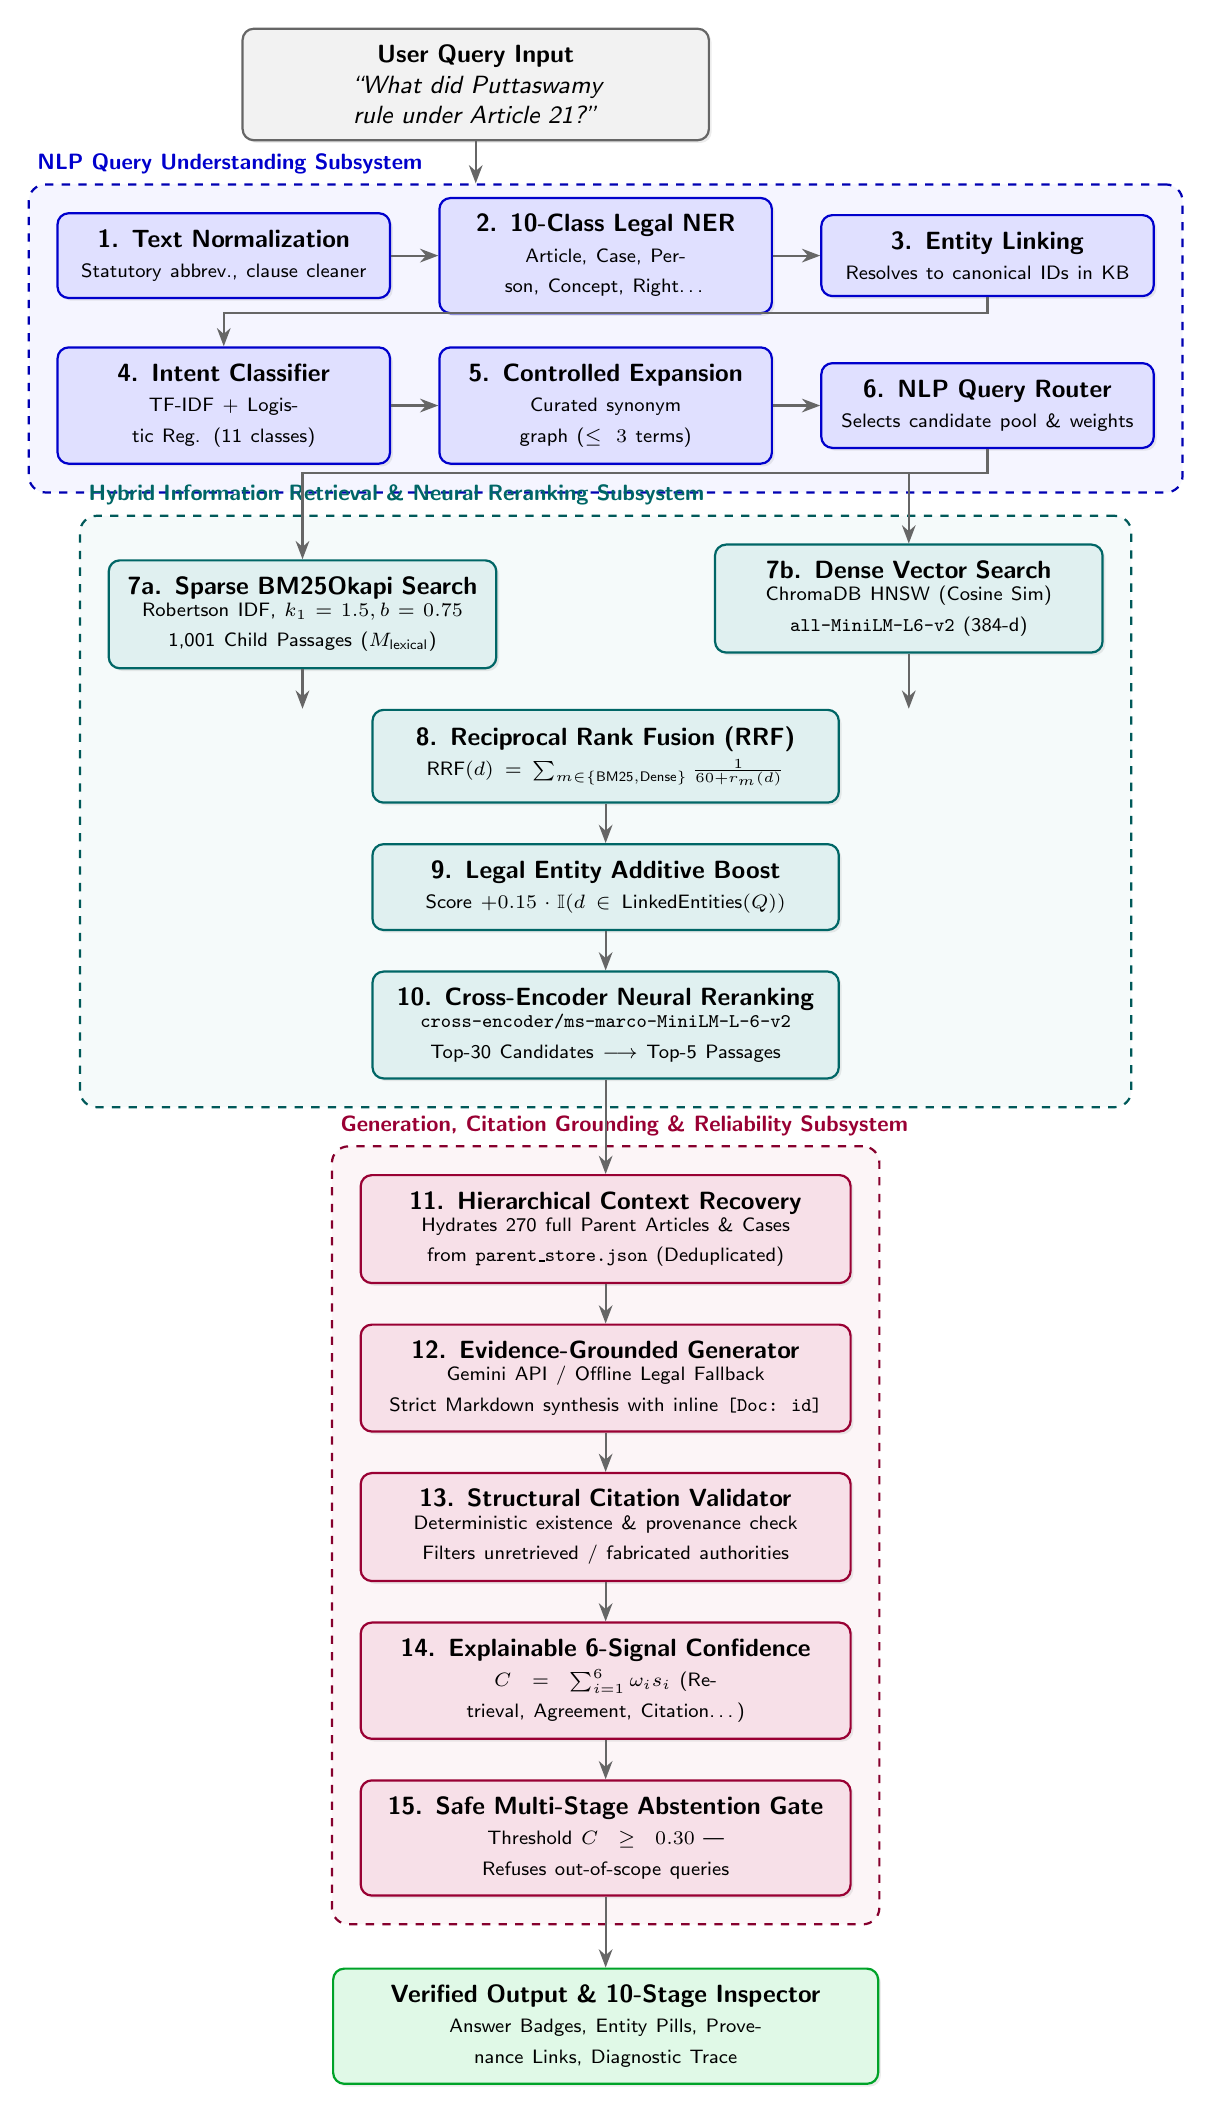
\begin{tikzpicture}[
    font=\sffamily\small,
    >=Stealth,
    node distance=0.75cm and 0.65cm,
    box/.style={rectangle, draw=#1!80!black, fill=#1!12, rounded corners=4pt, thick, align=center, inner sep=6pt, drop shadow={opacity=0.15, shadow xshift=1pt, shadow yshift=-1pt}},
    subsys/.style={rectangle, draw=#1!70!black, fill=#1!4, rounded corners=6pt, dashed, thick, inner sep=10pt},
    header/.style={font=\sffamily\bfseries\footnotesize, text=#1!80!black, align=center},
    flow/.style={->, thick, draw=gray!80!black},
    dataflow/.style={->, thick, dashed, draw=blue!70!black}
]

% Top: Query Input
\node[box=gray, text width=5.5cm, fill=gray!10] (query) {
    \textbf{User Query Input}\\
    \textit{``What did Puttaswamy rule under Article 21?''}
};

% Subsystem 1: NLP Query Understanding
\node[box=blue, text width=3.8cm, below=0.9cm of query, xshift=-3.2cm] (norm) {
    \textbf{1. Text Normalization}\\
    \scriptsize Statutory abbrev., clause cleaner
};

\node[box=blue, text width=3.8cm, right=0.6cm of norm] (ner) {
    \textbf{2. 10-Class Legal NER}\\
    \scriptsize Article, Case, Person, Concept, Right\dots
};

\node[box=blue, text width=3.8cm, right=0.6cm of ner] (el) {
    \textbf{3. Entity Linking}\\
    \scriptsize Resolves to canonical IDs in KB
};

\node[box=blue, text width=3.8cm, below=0.6cm of norm] (intent) {
    \textbf{4. Intent Classifier}\\
    \scriptsize TF-IDF + Logistic Reg. (11 classes)
};

\node[box=blue, text width=3.8cm, right=0.6cm of intent] (qe) {
    \textbf{5. Controlled Expansion}\\
    \scriptsize Curated synonym graph ($\le 3$ terms)
};

\node[box=blue, text width=3.8cm, right=0.6cm of qe] (router) {
    \textbf{6. NLP Query Router}\\
    \scriptsize Selects candidate pool \& weights
};

\begin{scope}[on background layer]
    \node[subsys=blue, fit=(norm) (el) (intent) (router)] (nlp_box) {};
    \node[header=blue, anchor=south west] at (nlp_box.north west) {NLP Query Understanding Subsystem};
\end{scope}

% Subsystem 2: Information Retrieval
\node[box=teal, text width=4.5cm, below=1.2cm of intent, xshift=1.0cm] (bm25) {
    \textbf{7a. Sparse BM25Okapi Search}\\
    \scriptsize Robertson IDF, $k_1=1.5, b=0.75$\\
    \scriptsize 1,001 Child Passages ($M_{\text{lexical}}$)
};

\node[box=teal, text width=4.5cm, below=1.2cm of router, xshift=-1.0cm] (dense) {
    \textbf{7b. Dense Vector Search}\\
    \scriptsize ChromaDB HNSW (Cosine Sim)\\
    \scriptsize \texttt{all-MiniLM-L6-v2} (384-d)
};

\node[box=teal, text width=5.5cm, below=0.6cm of $(bm25.south)!0.5!(dense.south)$] (rrf) {
    \textbf{8. Reciprocal Rank Fusion (RRF)}\\
    \scriptsize $\text{RRF}(d) = \sum_{m \in \{\text{BM25},\text{Dense}\}} \frac{1}{60 + r_m(d)}$
};

\node[box=teal, text width=5.5cm, below=0.5cm of rrf] (boost) {
    \textbf{9. Legal Entity Additive Boost}\\
    \scriptsize Score $+ 0.15 \cdot \mathbb{I}(d \in \text{LinkedEntities}(Q))$
};

\node[box=teal, text width=5.5cm, below=0.5cm of boost] (rerank) {
    \textbf{10. Cross-Encoder Neural Reranking}\\
    \scriptsize \texttt{cross-encoder/ms-marco-MiniLM-L-6-v2}\\
    \scriptsize Top-30 Candidates $\longrightarrow$ Top-5 Passages
};

\begin{scope}[on background layer]
    \node[subsys=teal, fit=(bm25) (dense) (rerank)] (ir_box) {};
    \node[header=teal, anchor=south west] at (ir_box.north west) {Hybrid Information Retrieval \& Neural Reranking Subsystem};
\end{scope}

% Subsystem 3: Generation & Reliability
\node[box=purple, text width=5.8cm, below=1.2cm of rerank] (parent_rec) {
    \textbf{11. Hierarchical Context Recovery}\\
    \scriptsize Hydrates 270 full Parent Articles \& Cases\\
    \scriptsize from \texttt{parent\_store.json} (Deduplicated)
};

\node[box=purple, text width=5.8cm, below=0.5cm of parent_rec] (gen) {
    \textbf{12. Evidence-Grounded Generator}\\
    \scriptsize Gemini API / Offline Legal Fallback\\
    \scriptsize Strict Markdown synthesis with inline \texttt{[Doc: id]}
};

\node[box=purple, text width=5.8cm, below=0.5cm of gen] (val) {
    \textbf{13. Structural Citation Validator}\\
    \scriptsize Deterministic existence \& provenance check\\
    \scriptsize Filters unretrieved / fabricated authorities
};

\node[box=purple, text width=5.8cm, below=0.5cm of val] (conf) {
    \textbf{14. Explainable 6-Signal Confidence}\\
    \scriptsize $C = \sum_{i=1}^6 \omega_i s_i$ (Retrieval, Agreement, Citation\dots)
};

\node[box=purple, text width=5.8cm, below=0.5cm of conf] (abst) {
    \textbf{15. Safe Multi-Stage Abstention Gate}\\
    \scriptsize Threshold $C \ge 0.30$ | Refuses out-of-scope queries
};

\begin{scope}[on background layer]
    \node[subsys=purple, fit=(parent_rec) (abst)] (rag_box) {};
    \node[header=purple, anchor=south west] at (rag_box.north west) {Generation, Citation Grounding \& Reliability Subsystem};
\end{scope}

% Bottom: UI / Output
\node[box=green!60!teal, text width=6.5cm, below=0.9cm of abst] (out) {
    \textbf{Verified Output \& 10-Stage Inspector}\\
    \scriptsize Answer Badges, Entity Pills, Provenance Links, Diagnostic Trace
};

% Connecting Arrows
\draw[flow] (query) -- (nlp_box.north -| query);
\draw[flow] (norm) -- (ner);
\draw[flow] (ner) -- (el);
\draw[flow] (el.south) -- ++(0,-0.2) -| (intent.north);
\draw[flow] (intent) -- (qe);
\draw[flow] (qe) -- (router);

\draw[flow] (router.south) -- ++(0,-0.3) -| (bm25.north);
\draw[flow] (router.south) -- ++(0,-0.3) -| (dense.north);

\draw[flow] (bm25.south) -- ++(0,-0.2) -| (rrf.north -| bm25.south);
\draw[flow] (dense.south) -- ++(0,-0.2) -| (rrf.north -| dense.south);
\draw[flow] (rrf) -- (boost);
\draw[flow] (boost) -- (rerank);

\draw[flow] (rerank) -- (parent_rec);
\draw[flow] (parent_rec) -- (gen);
\draw[flow] (gen) -- (val);
\draw[flow] (val) -- (conf);
\draw[flow] (conf) -- (abst);
\draw[flow] (abst) -- (out);

\end{tikzpicture}
\end{document}
